\documentclass[12pt]{standalone}
\usepackage{tikz}
\usetikzlibrary{decorations.pathreplacing}
\usetikzlibrary{decorations.markings}
\usetikzlibrary{positioning}
\usetikzlibrary{shapes}
\usetikzlibrary{calc}

\begin{document}
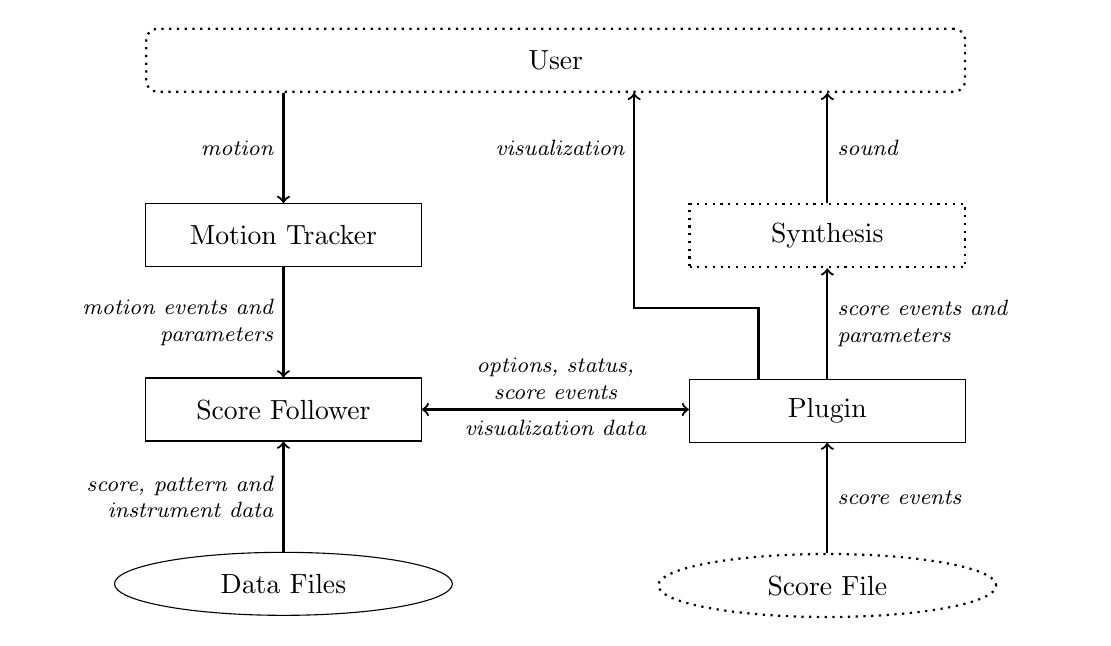
\begin{tikzpicture}

\IfStandalone {\tikzstyle{subtle}=[thin,gray]
\tikzstyle{subtle line}=[thin,gray!60]} {\tikzstyle{subtle}=[thin,gray]
\tikzstyle{subtle line}=[thin,gray!60]}

\def\BoxWidth{3.5cm}
\def\BoxHeight{0.8cm}
\def\Spacing{1.4cm}
\def\HSpacing{3.4cm}

% Styles
\tikzstyle{box} =
	[text centered, text width=0.8 * \BoxWidth, minimum width=\BoxWidth]

\tikzstyle{module} =
	[box, draw, minimum height=\BoxHeight]

\tikzstyle{outside} =
	[dotted, thick]

% Modules

\node (User) at (0, 0)
	[module, rounded corners, outside, minimum width=2*\BoxWidth+\HSpacing]
	{ User };
	
\path (User.south west) + (0, -\Spacing)
	node (MotionTracker) [module, anchor=north west] {Motion Tracker};
\node (ScoreFollower) [module, below=\Spacing of MotionTracker] {Score Follower};
\node (DataFiles) [module, ellipse, below=\Spacing of ScoreFollower] {Data Files};

\path (User.south east) + (0, -\Spacing)
	node (Synthesis) [module, outside, anchor=north east] {Synthesis};
\node (Plugin) [module, below=\Spacing of Synthesis] {Plugin};
\node (MIDIFile) [module, ellipse, outside, below=\Spacing of Plugin] {Score File};

% Edges

\tikzstyle{data text} =
	[font=\footnotesize\itshape]
	
\def\EdgeTextWidth{3cm}

\path[->, thick, data text, align=flush right, text width=\EdgeTextWidth]
	(User.south -| MotionTracker) edge node[left] (MotionNode) {motion} (MotionTracker)
	(MotionTracker) edge node[left] {motion events and parameters} (ScoreFollower)
	(DataFiles) edge
		node[left] {score, pattern and instrument data}
		(ScoreFollower);

\path[->, thick, data text, align=flush left, text width=\EdgeTextWidth]
	(MIDIFile) edge node[right] {score events} (Plugin)
	(Plugin) edge node[right] {score events and parameters} (Synthesis)
	(Synthesis) edge node[right] {sound} (User.south -| Synthesis);
	
\path[<->, thick, data text, align=center, text width=0.9*\HSpacing]
	(ScoreFollower) edge
	node[above] (SfPluginNode) {options, status, score events}
	node[below] {visualization data}
	(ScoreFollower -| Plugin.west);

\path
	let \p1 = (SfPluginNode.north),
	    \p2 = (Synthesis.south) in
	(\x1 + 1.0cm, {(\y1 + \y2) / 2}) node[coordinate] (VisualizationCorner) {};
\path[->, thick, draw, data text]
	let \p1 = (VisualizationCorner),
	    \p2 = (User.south) in
	(Plugin.north) +(-0.25 * \BoxWidth ,0)
	|- (\p1)
	-- (\x1, \y2);
	
\path[data text, align=flush right, text width=\EdgeTextWidth]
	let \p1 = (VisualizationCorner),
	    \p2 = (MotionNode) in
	(\x1, \y2) node[left] {visualization};


\end{tikzpicture}
\end{document}
